%%%%%

\documentclass[review,3p,times,12pt,number]{elsarticle}\usepackage{amsmath}\usepackage{amssymb}




\usepackage{multicol,enumitem,multirow,booktabs,amsthm,subfigure,rotating}
\usepackage{pdflscape}


\newlength{\smalltable}
\setlength{\smalltable}{252pt}


\newtheorem{proposition}{Proposition}
\newtheorem{definition}{Definition}


\usepackage[vlined,ruled,linesnumbered]{algorithm2e}
\SetKwComment{tcp}{/\!/\,}{}
\SetArgSty{textrm}
\SetKwProg{Procedure}{procedure}{}{end~procedure}
\SetKwProg{Function}{function}{}{end~function}
\SetKwFor{Repeat}{repeat}{times do}{end~loop}
\SetKwFunction{Move}{Move}
\SetKwFunction{Relocate}{Relocate}
\SetKwFunction{EvalMove}{EvalMove}
\SetKwFunction{Valid}{ValidTasks}
\SetKwFunction{Largest}{LargestPriorityTasks}
\SetKwFunction{EvalTask}{EvalTask}
\SetKwFunction{MoveNeed}{MoveNeed}
\SetKwFunction{Fill}{Fill}
\SetKwFunction{BiReceiver}{BiReceiver}
\SetKwFunction{BiSender}{BiSender}
\SetKwFunction{Interim}{Interim}
\SetKwFunction{InterimFull}{InterimFull}
\SetKw{Break}{break~while}

\renewcommand{\citet}[1]{\citeauthor{#1} \citep{#1}}
\makeatletter
\def\NAT@def@citea{\def\@citea{\NAT@separator}}
\makeatother

\usepackage[colorlinks=true]{hyperref}



\usepackage{caption}
\captionsetup[figure]{font=small}
\captionsetup[table]{skip=0.5ex,font=small}



\renewcommand{\gets}{\coloneqq}
\renewcommand{\emph}[1]{\textbf{\textit{#1}}}



\newcommand{\mss}{s^\mathrm{src}}
\newcommand{\mds}{s^\mathrm{dst}}
\newcommand{\mts}{s^\mathrm{tmp}}




\newcommand{\setalgo}{\linespread{1}\fontsize{10}{12}\selectfont}
\newcommand{\settab}{\linespread{1}\fontsize{10}{12}\selectfont}

\sloppy


\begin{document}

\begin{frontmatter}

\journal{EJOR}
\title{A feasibility-based heuristic for the container pre-marshalling problem}
\author[shu]{Ning Wang}
\ead{ningwang@shu.edu.cn}



\author[cityu]{Bo Jin\corref{cor}}
\ead{msjinbo@cityu.edu.hk}

\author[syu]{Zizhen Zhang}
\ead{zhangzizhen@gmail.com}

\author[nus]{Andrew Lim}
\ead{alim.china@gmail.com}
\cortext[cor]{Corresponding author.}

\address[shu]{Department of Information Management, School of Management, Shanghai University, Shanghai, China}
\address[cityu]{Department of Management Sciences, City University of Hong Kong, Hong Kong}
\address[syu]{School of Data and Computer Science, Sun Yat-Sen University, China}
\address[nus]{Department of Industrial \& Systems Engineering, National University of Singapore, Singapore}

\begin{abstract}

This paper addresses the container pre-marshalling problem (CPMP) which rearranges containers inside a storage bay to a desired layout.
By far, target-driven algorithms have relatively good performance among all algorithms; they have two key components: first, containers are rearranged to their desired slots one by one in a certain order; and second, rearranging one container is completed by a sequence of movements. Our paper improves the performance of the target-driven algorithm from both aspects.
The proposed heuristic determines the order of container rearrangements by the concepts of state feasibility, container stability, dead-end avoidance and tier-protection proposed in this paper.
In addition, we improve the efficiency of performing container rearrangements by discriminating different task types.
Computational experiments showcase that the performance of the proposed heuristic is considerable.
\end{abstract}

\begin{keyword}
container pre-marshalling problem \sep feasibility-based heuristic \sep tier-protection
\end{keyword}
\end{frontmatter}




\section{Introduction}



Since the commencement of containerization, the global use of standardized containers has dramatically improved international trade. Containers enable the smooth flow of goods between multiple transportation modes without directly handling the freight. Over the years, stringent requirements from consignors such as just-in-time operations have created challenges for the container transportation industry.

Container yards -- the space dedicated to the transshipment, handover, loading, consolidation, maintenance, and storage of containers -- are key components of maritime container terminals. Some yards act as exchange venues for container transfers between different transportation modes while others are used as caches for temporary storage or as warehouses for long-term storage.

Generally speaking, a container yard is divided into several yard blocks, each of which consists of several parallel bays.  A bay is formed by a row of stacks. Usually the containers stored in the same bay have the same dimensions. Equipments such as rubber tyre gantry cranes, rail-mounted gantry cranes, and reach stackers are frequently used in container yards. Figure \ref{fig:block} illustrates an example of a yard block.

\begin{figure}[htbp]
\centering
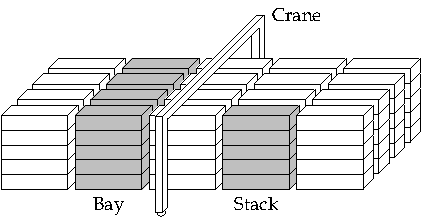
\includegraphics{figs/block.pdf}
\caption{Yard block.}
\label{fig:block}
\end{figure}

Containers in the same stack are operated in a last-in-first-out manner. To retrieve containers placed in lower tiers, containers on top of them must be relocated to other slots first. Such forced movements are known as container reshuffles or relocations.
Container pre-marshalling addresses the reorganization of containers inside a storage area such that no reshuffle is further required when containers are retrieved. Hence, the aim of pre-marshalling is to improve terminals' performance level, including throughput rate per berth and turnaround time of vessels or road trucks \citep{kim2015}.

The container pre-marshalling problem (CPMP) can be formally defined as follows. Containers are categorized into various groups, and each group is assigned with a group value. Given an initial layout of containers in a single bay, the CPMP aims at rearranging containers within the bay, such that containers in each stack are placed in a descending order of group values from the bottom up.
The objective of CPMP is to find the best container rearrangement plan with the fewest number of container movements.
It is assumed that the future retrieval order of containers is known beforehand and no container arrives at or leaves from the bay during pre-marshalling.

This paper designs a constructive heuristic which can be embedded later into frameworks such as beam search, large neighborhood search (LNS) and the greedy randomized adaptive search procedure (GRASP).
Our work makes three main contributions to the literature.
The first contribution is the concept of state feasibility. A set of rules are proposed for checking the feasibility of the states during the pre-marshalling process.
The feasibility of rearranging a certain container is checked before we actually conduct the rearrangement, which guarantees search efficiency.
The time complexity of checking the feasibility is only $\mathcal O(G)$; here $G$ is the number of groups. Our paper is the first work that applies feasibility to prune branches in CPMP algorithms.
The second contribution lies in the new techniques proposed: container stability, dead-end avoidance and tier-protection indicator, which foster better heuristic decisions.
The third contribution is the improvement of single container rearrangement which is achieved based on the relationship between the number of available slots and that of the blocking containers. This improvement avoids unnecessary container movements in certain situations.

The remainder of this paper is structured as follows. Section \ref{sec:literature} reviews existing approaches in the literature. Section \ref{sec:problem} formally describes the problem and lists the notation used throughout this paper. The concepts of state, state feasibility and container stability are introduced in Section \ref{sec:state}.
The proposed heuristic and the associated techniques are explained in Section \ref{sec:fbh}. Section \ref{sec:experiment} illustrates the experimental results of benchmark instances, and Section \ref{sec:conclusion} concludes this paper and identifies future research directions.

\section{Recent work}
\label{sec:literature}

According to recent reviews \citep{carlo2014,lehnfeld2014}, problems related to or caused by container reshuffles at terminals include three major types of decision problems. The first problem is the container relocation problem \citep{Jovanovic2014achain,jin2015} which minimizes the total operational cost in the container retrieval process. The operational cost is commonly measured by the number of relocations conducted or the total operational time. The second is the container pre-marshalling problem that is addressed in this paper. The third problem is the container stacking problem which decides the storage locations or crane operations for arriving containers \citep{Dayama2014}. All of the three problems are closely related and the solution methodologies have some common merits.



To the best of our knowledge, works that study the solutions to the CPMP are rather limited compared to other problems related to terminals. For example, berth allocation problems and quay crane scheduling problems have been studied by more than 120 publications just since 2009 \citep{Bierwirth2015}. One reason of limited works is that the variants of the CPMP by far are few. Known CPMP variants were studied by \citet{wang2015} who considered truck lanes, \citet{rendl2013} who allowed for group ranges rather than group values, and \citet{Huang2012} who required that containers of different groups be separately located in the final layout.



\citet{lee2007} developed an integer programming model for the CPMP\@. In their work, the problem was formulated as the multi-commodity network flow problem. The overall network is divided into several subnetworks, with each subnetwork representing an intermediate layout. The nodes in a subnetwork correspond to the slots that accommodate containers, and the commodities correspond to the containers stored in the bay. Every valid flow in the network represents a solution to the CPMP\@. The model provides an innovative viewpoint to see the problem, however, its performance is not good because the network is too large even for a small instance.

A neighborhood search was proposed by \citet{lee2009}, which repeatedly modifies the current solution until some termination condition is met. Unlike other existing solution-construction approaches, the neighborhood search is required to start with a pre-generated initial solution.
A feasible solution is further improved by a four-step procedure, and the diversity of the neighborhood is raised by multiple subroutines. The main drawback of the approach is the unreliability of random solution modifications, i.e., the feasibility of the new resultant solution is not always ensured.

\citet{bort2012} described a tree search procedure for solving the problem.
In the tree search procedure, solutions are constructed by compound moves instead of single moves. Moves are classified into four types, and only the most promising ones are adopted in the branching scheme. \citet{tierney2014} realized an A* algorithm with symmetry breaking rules, and \citet{van2014} presented an exact algorithm based on the branch and bound.


\citet{cas2009} provided a greedy heuristic named the corridor method for solving the problem. The heuristic selects the direction of movements in a randomized manner according to the attractiveness of available successors confined by the corridor.
A local improvement procedure was also conducted to accelerate the heuristic process.
\citet{exp2012} provided the first group-oriented heuristic for the CPMP\@. Their method iteratively handles containers in a descending order of group values. After handling all containers with a specific group value, a stack filling process was applied to reduce the number of disorderly containers in the bay.
\citet{jovanovic2014} developed a new method which designs different heuristics for each of the four stages of \citet{exp2012}.
\citet{wang2015} proposed a target-guided heuristic and two beam search algorithms.
The processes of determining container handling sequence and handling particular containers are both improved.
This work can solve instances of different densities well, especially dense instances with very few empty slots.
\citet{Gheith2014} proposed a rule-based heuristic procedure for solving the problem, and then developed a variable chromosome length genetic algorithm \citep{Gheith2015}.


\section{Problem description and notation}
\label{sec:problem}

The CPMP is restricted to the bay size, or more precisely, the dimensions of the operating cranes. A problem instance (problem input) includes an initial layout of $N$ containers, which are distributed in a single bay with $S$ stacks ($S\ge 3$) and $H$ tiers ($H\ge 2$) with $E$ empty slots ($E=SH-N$, $E\ge 2$) left.

Every container is labeled a group value $g \in\{1,\dots,G\}$. A container is \emph{orderly} if it is supported directly by the ground or another orderly container with equal or larger group value; otherwise, it is \emph{disorderly}. Other phrases in the recent literature that have the same meaning of ``orderly{\slash}disorderly''  include ``well{\slash}badly placed'' \citep{bort2012}, ``well-{\slash}non-located'' \citep{exp2012}, and ``clean{\slash}dirty'' \citep{wang2015}.

Figure \ref{fig:bay} gives an example of a bay with $S=5$, $H=4$, and $N=13$. Containers are represented by boxes with their group values marked inside.
Specially, disorderly containers are highlighted by gray backgrounds.
The objective of the CPMP is to find an optimized sequence with the fewest container movements. By applying the obtained movement sequence to the initial layout, all the containers could be rearranged to be orderly.

\begin{figure}[htbp]
\centering
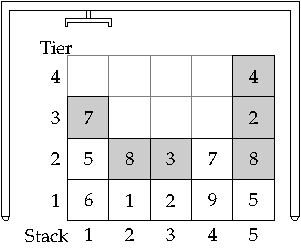
\includegraphics{figs/bay.pdf}
\caption{A container bay.}
\label{fig:bay}
\end{figure}


To better describe the solution to the CPMP, layout-related notation is introduced first.
Stacks and tiers of the bay are labeled from left to right and bottom to top, respectively.
Let $\mathbb{S}=\{1,\dots,S\}$ be the set of stacks. Hereafter, for simplification of description, when a stack $s$ is mentioned without declaring its domain, it is assumed that $s\in\mathbb{S}$. The height of stack $s$ is denoted by $h(s)$ and $e(s)=H-h(s)$ denotes the number of empty slots in stack $s$. Note that the height of stacks should not exceed $H$.
The orderly height (number of orderly containers) of stack $s$ is denoted by $o(s)$.
The slot positioned at the $t$-th tier of stack $s$ is denoted by $(s,t)$.
The group value of a container $c$ is denoted by $g(c)$.
Moreover, the group value of a container located in slot $(s,t)$ is denoted by $g(s,t)$.







\section{State and state feasibility}
\label{sec:state}

\begin{definition}[Fixed containers]
A fixed container is an orderly container which has been locked to a certain slot. Fixed containers are not allowed to be moved in subsequent movements.
\end{definition}

According to the definition of fixed containers,  fixed containers in the same stack are contiguous from the bottom up.

\begin{definition}[State]
A state $(\mathsf{L},\boldsymbol{f})$ is a two-tuple composed of a layout $\mathsf{L}$ and a fix vector $\boldsymbol{f}$.
\end{definition}

The fix vector $\boldsymbol{f}$ indicates the fixed height (number of fixed containers) of each stack of the layout $\mathsf{L}$. The $s$-th element of $\boldsymbol{f}$ is denoted by $f(s)$.

Figure \ref{fig:skyline} illustrates two examples of state, where fixed and unfixed containers are separated by \emph{skylines} (bold lines).
In Figure \ref{fig:exp1}, $\boldsymbol f=(2,3,1)$; in Figure \ref{fig:exp2}, $\boldsymbol f=(2,3,0)$.

\begin{figure}[htbp]
\centering
\subfigure[]{
    \label{fig:exp1}
    \resizebox{0.35\textwidth}{!}{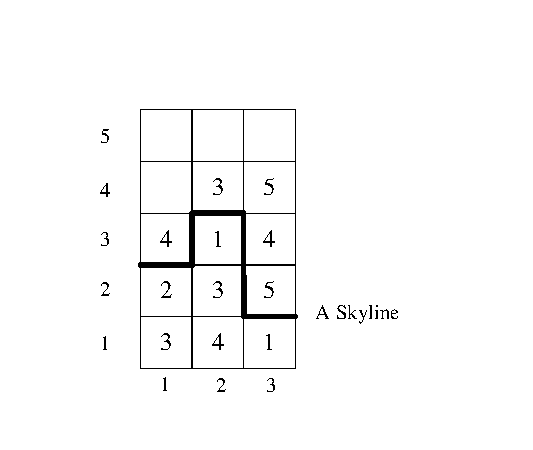
\includegraphics{figs/exp1.pdf}}}
\subfigure[]{
    \label{fig:exp2}
    \resizebox{0.35\textwidth}{!}{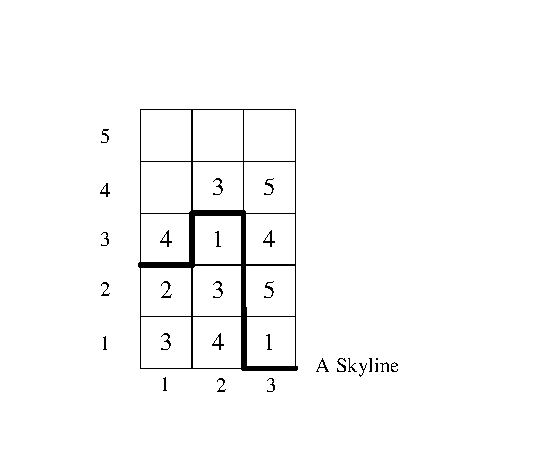
\includegraphics{figs/exp2.pdf}}}
\caption{State, fixed vector and skyline.}
\label{fig:skyline}
\end{figure}


It is noteworthy that if two states have the same layout but different fix vectors, then they are two different states, just like Figures \ref{fig:exp1} and \ref{fig:exp2}.

\begin{definition}[Feasibility of a state]
A state $(\mathsf{L},\boldsymbol{f})$ is feasible if there exists a movement sequence that can convert $\mathsf{L}$ to an orderly layout without moving fixed containers indicated by $\boldsymbol{f}$.
\end{definition}

The necessary condition for state feasibility has been talked about in \citet{wang2014}. To make the content self-contained, we briefly explain it in this paper. Containers above the skyline can be moved, therefore slots and containers above the skyline are separately considered.

For a stack $s$ in state $(\mathsf{L},\boldsymbol{f})$, suppose that the smallest group value under the skyline is $g$, then there are $H-f(s)$ slots above the skyline which can only be filled with containers $c$ such that $g(c)\le g$. In such a situation, we say stack $s$ has $H-f(s)$ slots with capability $g$.
If the skyline of stack $s$ coincides with the ground, then stack $s$ has $H$ slots with capability $G$.
For example, in Figure \ref{fig:exp2}, stack 1, 2 and 3 have 3, 2 and 5 slots with capabilities 2, 1 and 5, respectively. The total number of slots with capability $g$ in the whole bay is denoted by $r(g)$ (resource for group $g$).
Similarly, the number of unfixed containers with group value $g$ is denoted by $d(g)$ (demand of group $g$).

In a feasible state, the slots available for group $g$ (i.e., slots with capabilities no smaller than $g$) must exceed the demand of group $g$. That is,
\begin{equation*}
\sum^G_{i=g+1}r(i)-\sum^G_{i=g+1}d(i)+r(g)\ge d(g),
\end{equation*}
which is equivalent to
\begin{equation*}
\sum^G_{i=g}r(i)\ge \sum^G_{i=g} d(i).
\end{equation*}

Denote $R(g)=\sum^G_{i=g}r(i)$ and $D(g)=\sum^G_{i=g}d(i)$, then $\boldsymbol R$ and $\boldsymbol D$ are the two $G$-dimensional vectors with elements $R(g)$ and $D(g)$, respectively. The above condition can be hence expressed as $\boldsymbol{\Delta}=\boldsymbol{R}-\boldsymbol{D}\ge \boldsymbol{0}$. Here, $\boldsymbol \Delta$ is called the \emph{surplus vector}.



\begin{proposition}[Necessary condition for state feasibility]
$\boldsymbol{\Delta}=\boldsymbol{R}-\boldsymbol{D}\ge \boldsymbol{0}$ is a necessary condition for a feasible state $(\mathsf{L},\boldsymbol{f})$.
\end{proposition}



Take the two states in Figures \ref{fig:exp1} and \ref{fig:exp2} as examples.
Table \ref{tab:feasible} shows the surplus vectors for both states. State $a$ is infeasible since $\Delta(g)<0$ for $g=2,\dots,5$. It is intuitively seen that none of the stacks in Figure \ref{fig:exp1} can accommodate containers with group value 5, and this is the reason why state $a$ is infeasible.
The feasibility of state $b$ is not sure yet because $\boldsymbol{\Delta}\ge \boldsymbol {0}$ is only a necessary condition. Note that the time complexity of checking $\boldsymbol{\Delta}\ge \boldsymbol{0}$ is $\mathcal O(G)$.

\begin{table}[htbp]
\caption{Computation of the surplus vector.}
\centering

\begin{tabular}{|c|c|c|c|c|c| c |c|c|c|c|c|c|}
\cline{1-6}
\cline{8-13}
\multicolumn{6}{|c|}{State $a$} & \multicolumn{1}{c}{}& \multicolumn{6}{|c|}{State $b$}\\
\cline{1-6}
\cline{8-13}
$g$ & $d(g)$ & $D(g)$ & $r(g)$ & $R(g)$ & $\Delta(g)$ && $g$ & $d(g)$ & $D(g)$ & $r(g)$ & $R(g)$ & $\Delta(g)$\\
\cline{1-6}
\cline{8-13}
1   & 0      & 5      & 6      & 9      & 3           && 1   &  1     & 6       & 2      & 10     & 4\\
2   & 0      & 5      & 3      & 3      & -2          && 2   &  0     & 5       & 3      & 8      &  3\\
3   & 1      & 5      & 0      & 0      & -5          && 3   &  1     & 5       & 0      & 5      &  0\\
4   & 2      & 4      & 0      & 0      & -4          && 4   &  2     & 4       & 0      & 5      &  1\\
5   & 2      & 2      & 0      & 0      & -2          && 5   &  2     & 2       & 5      & 5      &  3\\
\cline{1-6}
\cline{8-13}
\end{tabular}
\label{tab:feasible}
\end{table}



\begin{definition}[Container stability]
Consider a given feasible state. Disorderly containers are unstable. For any orderly container $c$ in slot $(s,t)$, try to fix container $c$ and those underneath. If the resultant state has $\boldsymbol{\Delta}\ge 0$, then $c$ is stable; otherwise, $c$ is unstable.
\end{definition}

According to the definition, an unstable container is not allowed to be fixed in the current slot even if it is orderly, because the resultant state would be infeasible.
Unstable containers must be moved in the future. Denote the stable height (number of stable containers) of stack $s$ by $\mathit{sh}(s)$, then we have $\boldsymbol{f}\le \boldsymbol{\mathit{sh}}\le \boldsymbol{o}\le \boldsymbol{h}$. If a container $c$ could become stable by moving it onto stack $s$, we say that stack $s$ can \emph{stabilize} $c$.

Figure \ref{fig:stable} gives another example of a state. Fixed containers are labeled with solid squares and unstable containers are highlighted in gray backgrounds. Notice that the container in slot $(2,1)$ with group value $6$ is orderly but unstable.

\begin{figure}[htbp]
\centering
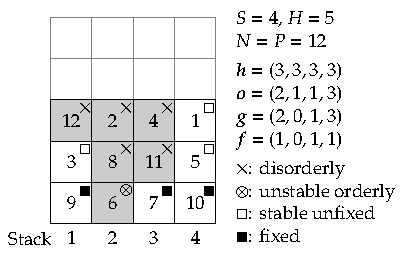
\includegraphics{figs/stable.pdf}
\caption{Stability of containers.}
\label{fig:stable}
\end{figure}

An orderly but unstable container indicates that its orderliness is valueless because it definitely requires at least one movement.
Using the concept of container stability instead of container orderliness is more precise in evaluating the movements of blocking containers during the pre-marshalling process.
For example, when deciding the next movement of a blocking container, if the container becomes orderly but unstable after being moved to a new stack, the attractiveness of such a movement should be reconsidered. The stability of containers should be recomputed after any container is fixed.



\begin{definition}[Extreme state]
A state $(\mathsf{L},\boldsymbol{f})$ is called an extreme state if $|\{s\in\mathbb{S}: f(s)=H\}|= S-2$.
\end{definition}

The definition of extreme state is to emphasize the special case where $S-2$ stacks are fully fixed. In such a case, unfixed containers can only be moved between the other two stacks, say $a$ and $b$. An extreme state is feasible if and only if one of the following conditions is satisfied:
\begin{enumerate}
\item Both stacks $a$ and $b$ are orderly;
\item Stack $a$ is orderly, and stack $b$ is disorderly. Stack $a$ is still orderly after all the disorderly containers of stack $b$ are moved to stack $a$.
\end{enumerate}

\begin{definition}[Dead-end state]
A state is called a dead-end state if it is an infeasible extreme state.
\end{definition}


We have the following proposition.

\begin{proposition}[Existence of dead-end states]
In extremely dense instances such that $E<2(H-1)$, there exist possibilities of generating a dead-end state, while in instances with $E\ge2(H-1)$, dead-end states will never be generated.
\end{proposition}

When $E\ge 2(H-1)$, it has $N\le SH-2H+2$. When fewer than $S-2$ stacks are fully occupied, the state is not a dead-end state; when $S-2$ stacks are fully occupied, there are at most two extra containers in the left two stacks. The state is not a dead-end state, either. 
Figure \ref{fig:non-dead-end} gives an example of an instance with $E\ge2(H-1)$, which has no chance to generate any dead-end state.

For instances with $E<2(H-1)$, there exist possibilities of generating a dead-end state.
Figure \ref{fig:dead-end} gives an example with $E<2(H-1)$; when $\boldsymbol f=(0,0,5,5)$, the corresponding state is a dead-end state.
\begin{figure}[htbp]
\centering
\subfigure[]{
    \label{fig:non-dead-end}
    \resizebox{0.2\textwidth}{!}{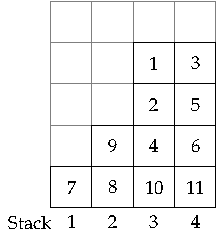
\includegraphics{figs/non-dead-end.pdf}}}
\subfigure[]{
    \label{fig:dead-end}
    \resizebox{0.2\textwidth}{!}{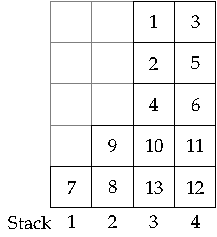
\includegraphics{figs/dead-end.pdf}}}
\caption{Existence of dead-end states.}
\end{figure}

\section{Feasibility-based heuristic}
\label{sec:fbh}

In this section, a feasibility-based heuristic (FBH) is developed for solving the CPMP\@. The proposed heuristic is a target-driven algorithm. Target-driven algorithms \citep{exp2012,wang2015} are efficient among all existing algorithms. Generally speaking, containers (targets) are rearranged to certain slots one by one, and each rearrangement is achieved by a sequence of movements.
The heuristic can be implemented independently as a greedy algorithm, or be a major component embedded in meta-heuristic frameworks.
In this paper, we optimize the order of container rearrangements as well as the sequence of movements in one rearrangement.

The optimization is partially due to the concept of state feasibility.
This is also the reason why our algorithm is called feasibility-based heuristic.
Before a certain container is rearranged, the feasibility of the resultant state is always ensured.
In other words, any rearrangement that leads to an infeasible state is eliminated.
Due to the state feasibility check, we can explore larger space without sacrificing efficiency. The order of container rearrangements is dynamically determined as the algorithm goes on.



\subsection{Heuristic framework}

According to \citet{wang2014}, in dense instances with $E<H$, only the top $\sum_{i\neq s}e(i)$ containers of a stack $s$ can be moved. The immovable number of containers (unreachable tiers) in any stack is $H-E$, i.e., containers in the lowest $H-E$ tiers of the bay are unreachable.
In loose instances such that $E\ge H$, all the containers are movable.
We define $U=\max\{H-E,0\}$ as the number of unreachable tiers for any instance.


The feasibility-based heuristic firstly constructs the initial state according to the unreachable tiers. In the initial state, $\mathsf{L}^0$ is the initial layout and containers in unreachable tiers are naturally fixed, i.e., the initial state is $(\mathsf{L}^0,U\cdot\boldsymbol{1})$, where $\boldsymbol 1$ is an $S$-dimensional all-ones vector.

Starting from the initial state, the heuristic repeatedly fixes a target container $c^*$ to an aim stack $s^*$.
Since stack $s^*$ already has $f(s^*)$ fixed containers, $c^*$ will be fixed at tier $f(s^*)+1$. The algorithm continues until all the containers are fixed. The procedure of the proposed heuristic is concisely described in Algorithm \ref{algo:fbh}.

\begin{algorithm}[htbp]
\caption{Feasibility-based heuristic.}
\label{algo:fbh}


\setalgo


\Begin
{
  $(\mathsf{L},\boldsymbol{f})\gets (\mathsf{L}^0,U\cdot\boldsymbol{1})$\;
  \Repeat{$N-SU$}
  {
    $(c^*\rightarrow s^*)\gets\textrm{the selected valid task}$\;
    $\mathsf{L} \gets \textrm{resultant layout after rearranging $c^*$ to stack $s^*$}$\;
    $f(s^*)\gets f(s^*)+1$\;
  }
}

\end{algorithm}

The procedures of selecting the next task $c^*\rightarrow s^*$ and rearranging $c^*$ to stack $s^*$ will be explained in Sections \ref{sec:task_sel} and \ref{sec:speedy}, respectively.

The advantage of fixing containers one by one lies in twofold.
\begin{enumerate}
\item Movements are more target-oriented. Some works such as \citet{bort2012} move a container each time, but they don't have a clear aim. Hence, it is difficult to measure the benefit of movements. Moreover, movements are blind: a container can be unnecessarily moved from stack $a$ to $b$ and then moved from $b$ to $a$ in later movements.
\item Unfixed containers are allowed to be moved, but fixed ones are not. The ``fixed/unfixed'' status can distinguish fixed containers and unfixed containers, especially unfixed orderly containers. In works that do not distinguish fixed and unfixed containers, containers that have been rearranged (``fixed'' in our context) still get involved in later movements.
\end{enumerate}

\subsection{Task selection}
\label{sec:task_sel}
\subsubsection{Valid task}
At every step of the heuristic, an unfixed container and a destination stack are determined as the target container and the aim stack, respectively.
Most target-driven algorithms select target containers according to a predetermined order, such as the descending order of group values \citep{exp2012}. In this research, the order to rearrange containers is not fixed beforehand, but rather dynamically decided as the algorithm goes on. This innovation undoubtedly enables the algorithm to explore larger solution space, but one may say that the search efficiency is reduced. To this end, the concept of state feasibility is applied to avoid useless solution space.
Our paper is the first work that applies state feasibility to prune branches in existing CPMP algorithms.

A container--stack pair $c\rightarrow s$ is a valid task for the current state $(\mathsf{L},\boldsymbol{f})$ only if
\begin{itemize}
\item $c$ is unfixed,
\item $f(s)<H$,
\item $g(c)\le g(s,f(s))$, and
\item $\Delta(\varphi)\ge H-f(s)$, for $\varphi\in (g(c),g(s,f(s))]$.
\end{itemize}
The first condition is easy to understand. The second condition ensures that stack $s$ has at least one slot to accommodate $c$.
The third condition makes sure that the group value of $c$ is not larger than $g(s,f(s))$.
The last condition ensures the non-negativity of the resultant surplus vector.
If $c$ is moved to stack $s$, then $d(g(c))$ (i.e., the demand of group $g(c)$) decreases by 1, that is, the demand of group $g(c)$ in the resultant layout is $d'(g(c))=d(g(c))-1$, while other elements of the demand vector are not changed.
Meanwhile, for the resource vector, $r'(g(s,f(s)))=r(g(s,f(s)))-(H-f(s))$, $r'(g(c))=r(g(c))+H-f(s)-1$, and other elements are not changed. Then for $\varphi\in (g(c),g(s,f(s))]$, the feasibility condition in the resultant layout is $D'(\varphi)=\sum_{g\ge \varphi}d'(g)=D(\varphi)\le R'(\varphi)=\sum_{g\ge\varphi}r'(g)=R(\varphi)-(H-f(s))$, which can be further simplified to $\Delta(\varphi)\ge H-f(s)$.

Container--stack pairs that satisfy the above conditions compose a set $\mathbb T$. However, the above conditions are only necessary conditions. The feasibility of the resultant state is still not ensured, due to the possibility of dead-end states.

There are three methods for resolving the issue of dead-end states.
\begin{enumerate}
\item Prevent from entering an extreme state when deciding the next task;
\item Design an ideal task accomplishment procedure that guarantees the feasibility of resultant states;
\item Allow entering a dead-end state and relabel a fixed container as unfixed to escape from the dead-end state.
\end{enumerate}

Our previous work \citep{wang2015} adopts the last method listed above. When the algorithm enters a dead-end state, the algorithm relabels a fixed container as unfixed and moves it to a temporary slot. After taking a sequence of movements, the relabeled container returns to the slot where it is originally fixed. The disadvantage of such a method is that escaping from the current dead-end state causes unnecessary movements. A better choice is to avoid resulting in dead-end states in advance when choosing valid tasks.

\begin{definition}[Pre-extreme state]
A feasible state is a pre-extreme state if $|\{i\in\mathbb{S}: f(i)=H\}|=S-3$, $|\{i\in\mathbb{S}: f(i)=H-1\}|\ge 1$ and $\sum_{i\in\mathbb{S}}f(i)<N-2$.
\end{definition}

The proposed heuristic only explores states $(\mathsf{L},\boldsymbol{f})$ which satisfy $\boldsymbol{\Delta}\ge \boldsymbol{0}$.
When $S-3$ stacks are fully fixed ($|i \in \mathbb S : f(i)= H| = S- 3$), and at least one stack has only one available slot left ($|i \in \mathbb S : f(i) = H-1| \ge 1$), let us investigate the validity of performing a task $c\rightarrow s$ with $f(s)=H-1$ based on the number of remaining unfixed containers.
\begin{enumerate}
\item If $\sum_{i\in\mathbb{S}} f(i) = N$, all the containers are fixed. The algorithm terminates with an orderly layout.

\item If $\sum_{i\in\mathbb{S}} f(i) = N-1$, it means that only one container $c$ remains unfixed. As $\boldsymbol{\Delta}\ge \boldsymbol {0}$, and $D(g(c))=d(g(c))=1$, we have $R(g(c))\ge1$, that is, there is at least one slot which can make $c$ orderly. At most one movement is needed to convert the layout to an orderly layout.

\item If $\sum_{i\in\mathbb{S}}f(i) = N-2$, two containers remain unfixed. Suppose the last two unfixed containers are $a$ and $b$, and the valid task is $a\rightarrow s$ with $f(s)=H-1$. Because $a\rightarrow s$ is a valid task, so the fourth condition ($\Delta(\varphi)\ge H-f(s)$, for $\varphi\in (g(c),g(s,f(s))]$) is satisfied. Therefore, the resultant layout satisfies $\boldsymbol \Delta' \ge \boldsymbol{0}$ and only $b$ remains unfixed in the resultant layout. Hence, performing task $a\rightarrow s$ does not result in a dead-end state.

\item If $\sum_{i\in\mathbb{S}} f(i)\le N-3$, at least 3 containers remain unfixed. If the next task is to fix a container to a stack $s$ with $f(s)=H-1$, the resultant layout might be a dead-end state. Taking Figure~\ref{fig:pre-extreme} as an example. Boxes with a solid square represent fixed containers. The task $1\rightarrow 3$ is valid since the surplus vector of the resultant state is non-negative, however, the resultant state is a dead-end state.
\end{enumerate}

\begin{figure}[htbp]
\centering
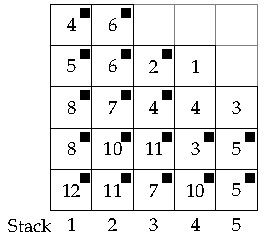
\includegraphics{figs/c.pdf}
\caption{Pre-extreme state.}
\label{fig:pre-extreme}
\end{figure}

Based on the above discussion, we can see that when $\sum_{i\in\mathbb{S}}f(i)<N-2$, there is danger to enter a dead-end state.

When the current state is a pre-extreme state, we immediately eliminate those container--stack pairs $c\rightarrow s$ with $f(s)=H-1$ from $\mathbb T$, so that the algorithm is able to avoid dead-end states. This technique is called ``dead-end avoidance''.

\subsubsection{Task evaluation}

Every valid task $c\rightarrow s$ in $\mathbb{T}$ is evaluated by a tuple with six elements:
\begin{enumerate}
\item the tier-protection indicator;
\item the number of movements required by the speedy task accomplishment procedure;
\item the number of stable containers that need to be moved from the aim stack;
\item the affected demand;
\item the fixed height of aim stack;
\item the negative of $g(c)$;
\end{enumerate}
The tuples of valid tasks are compared lexicographically, and the task with the minimum tuple is selected as the next task. The six elements in the tuple will be explained in the following.

The tier-protection indicator is to balance the trade-off between the freedom of task selection and the surplus loss. In principle, a container can be moved to any valid stack.
However, if a container with small group value occupies a relatively empty stack, then the loss of surplus vector is large: after the target container $c$ is fixed to the aim slot $(s,f(s)+1)$, the surplus $\Delta(\varphi)$ is reduced by $H-f(s)$, for $\varphi\in (g(c),g(s,f(s))]$.
The larger the gap between $g(c)$ and $g(s,f(s))$ is, the more the surplus vector will lose.
If a task $c\rightarrow s$ satisfies $f(s)\le P1$ and the affected demand $\sum_{\varphi=g(c)+1}^{g(s,f(s))}d(\varphi)\ge P2$,  the task is then deleted from $\mathbb{T}$. As two customizable parameters, the number of tiers protected $P1$ and the threshold value $P2$ can be adjusted optionally.

The number of moves required by the speedy task accomplishment procedure can be precisely computed in the proposed speedy task accomplishment procedure, which is an improvement of the estimation in \citet{wang2015}.
The process to compute the number of needed movements is introduced in Section \ref{sec:speedy}.

The number of stable containers that need to be moved from the aim stack is $\mathit{sh}(s)-f(s)$.
The affected demand is $\sum_{\varphi=g(c)+1}^{g(s,f(s))}d(\varphi)$.
The fixed height of aim stack $f(s)$ favors low tiers, which makes the fixed height of stacks even.
The last element $-g(c)$ prefers a target container with a larger group value.


\subsection{Speedy task accomplishment procedure}

\label{sec:speedy}
After a task is selected, a speedy task accomplishment procedure (STAP) is carried out to accomplish the task, resulting in a new state. The movement sequence of the STAP is based on task types.

Let $c^*$ denote the target container located in $(s^+,t^+)$ and $s^*$ denote the aim stack. The task is \emph{immediate} if $c^*$ is already on the highest fixed container of stack $s^*$, i.e., $s^+=s^*$ and $t^+=f(s^*)+1$;
the task is \emph{internal} if $c^*$ is above but not directly on the highest fixed container of stack $s^*$, i.e., $s^+=s^*$ and $t^+>f(s^*)+1$;
and the task is \emph{external} if $c^*$ is not in stack $s^*$ currently, i.e., $s^+\neq s^*$.


\subsubsection{Immediate task}

An immediate task does not require any move because the target container is already located in the aim slot.

\subsubsection{Internal task}

For an internal task, let $a$ denote the number of empty slots except those in stack $s^+$ and one highest non-full stack; that is, $a=E-e(s^+)-\min\{e(s):e(s)>0,s\neq s^+\}$.   Let $B_1$ ($b_1=|B_1|$) and $B_2$ ($b_2=|B_2|$) denote the sets (numbers) of blocking containers above and below $c^*$, respectively. Blocking containers refer to containers which blocks the target container or the aim slot.
The accomplishment procedure for an internal task is given in Algorithm \ref{algo:internal}.

\begin{algorithm*}[htbp]

\caption{Accomplish an internal task.}
\label{algo:internal}

\setalgo

\SetKwProg{One}{case I1:}{}{end~case}
\SetKwProg{Two}{case I2:}{}{end~case}
\SetKwProg{Three}{case I3:}{}{end~case}
\SetKwInput{Target}{target container}
\SetKwInput{Aim}{aim slot}
\SetKwInput{Above}{blocking above}
\SetKwInput{Below}{blocking below}
\SetKwInput{Slot}{slot supply}

\begin{multicols}{2}
\Target{$c^*(s^+,t^+)$}

\Aim{$(s^+,f(s^+)+1)$}
\Slot{$a=E-e(s^+)-\min\{e(s):e(s)>0,s\neq s^+\}$}

\Above{$b_1=h(s^+)-t^+$}
\Below{$b_2=t^+-f(s^+)-1$}
  \One{$a\ge b_2$}
  {
    \Repeat{$b_1$}
    {
      $\mathbb{R}\gets \{ s\neq s^+: h(s)<H,\, \alpha(s^+,s)\ge b_2\}$\;

      \Relocate{$s^+,1,\mathbb{R}$}\;
    }
    $\mathbb{I}\gets \{s\neq s^+: h(s)<H,\, E-e(s^+)-e(s)\ge b_2\}$\;

    $\mts\gets \Interim{$\mathbb{I}$}$\;
    \Move{$s^+,1,s'$}\;
    \Relocate{$s^+,b_2,\mathbb{S}\setminus\{s^+,\mts\}$}\;
    \Move{$\mts,1,s^+$}\;
    \tcp{I1:\ $h(s^+)-f(s^+)+1$ movements}
  }

  \Two{$a<b_2$ \& $|\{s\neq s^+: h(s)<H\}|>1$}
  {
    \Relocate{$s^+, b_1, \mathbb{S}\setminus\{s^+\}$}\;
    $\mts_1\gets \Interim{$\mathbb{S}\setminus\{s^+\}$}$\;
    \Move{$s^+, 1, \mts_1$}\;
    $k_2\gets E-e(s^+)-e(\mts_1)-1$\;
    \Relocate{$s^+, k_2, \mathbb{S}\setminus\{s^+,\mts_1\}$}\;
    Find $\mts_2$ s.t.\ $\mts_2\not\in \{s^+,\mts_1\}$ \& $h(\mts_2)<H$\;
    \Move{$\mts_1, 1, \mts_2$}\;
    \Move{$s^+, b_2-k_2, \mts_1$}\;
    \Move{$\mts_2, 1, s^+$}\;
    \tcp{I2:\ $h(s^+)-f(s^+)+2$ movements}
  }

  \Three{$a<b_2$ \& $|\{s\neq s^+: h(s)<H\}|=1$}
  {
    Find $s'$ s.t.\ $s'\neq s^+$ \& $h(s')<H$\;
    $\mts\gets \InterimFull{$\mathbb{S}\setminus\{s^+,s'\}$}$\;
    \BiSender{$\mts, 1, s^+, b_1, \{s'\}$}\;
    \Move{$s^+, 1, \mts$}\;
    \Move{$s^+, b_2, s'$}\;
    \Move{$\mts, 1, s^+$}\;
    \tcp{I3:\ $h(s^+)-f(s^+)+2$ movements}
  }

\end{multicols}
\BlankLine
\BlankLine
\end{algorithm*}

The accomplishment procedure is carried out based on the relationship between $a$ and $b_2$, which determines how containers are relocated.
\begin{itemize}
\item I1: $a\ge b_2$;
\item I2: $a<b_2$ \& $|\{s\neq s^+: h(s)<H\}|>1$;
\item I3: $a<b_2$ \& $|\{s\neq s^+: h(s)<H\}|=1$.
\end{itemize}

In case I1, $b_1$ containers above $c^*$ are relocated one by one. $\mathbb R$ represents the set of available destination stacks for the top container of stack $s^+$.
When relocating containers from $B_1$, reserving slots for containers from $B_2$ should be considered beforehand. Because $c^*$ is above $B_2$, so $c^*$ is relocated before containers of $B_2$.
If some movements put $c^*$ and $B_2$ in the same stack, then $c^*$ needs additional movements to be retrieved.

%The stack $s_\text{min}$ with the minimum number of empty slots is reserved for $c^*$. Therefore, containers of $B_2$ can only be placed at stacks $\{s\in S:s\neq s^+, s\neq s_\text{min}\}$.
When deciding whether a stack $s^{\text{dst}}$ can be the destination of a container $c$ from $B_1$, function $\alpha$ is used to compute how many slots will be left for $B_2$ after $c$ is placed to stack $s^{\text{dst}}$ .
If the left slots are not enough for $B_2$, $c$ cannot be moved to $s^{\text{dst}}$.
The pseudo-code of function $\alpha$ is given in Algorithm \ref{algo:alpha}.

\begin{algorithm}[htbp]

\caption{Function $\alpha$.}
\label{algo:alpha}
\setalgo
\begin{multicols}{2}
\Function{$\alpha(s^+,\mds)$}
        {\tcp{$s^+\neq \mds$}
            $e^{\min}\gets \min\{e(s)>0:s\neq s^+\}$\;
            $e^{\sec}\gets \min\{e(s)>e^{\min}:s\neq s^+\}$\;
            $k^{\min}\gets |\{s\neq s^+ : e(s)=e^{\min}\}|$\;
            \uIf{$e(\mds)> e^{\min}$}
            {
                \Return $E-e(s^+)-e^{\min}-1$\;
            }
            \uElseIf{$e^{\min}\ge 2$}
            {
                \Return $E-e(s^+)-e^{\min}$\;
            }
            \uElseIf{$k^{\min}=1$}
            {
                \Return $E-e(s^+)-e^{\sec}-1$\;
            }
            \Else
            {
                \Return $E-e(s^+)-2$\;
            }
        }
\end{multicols}
\BlankLine
\BlankLine
\end{algorithm}

If $e(\mds)> e^{\min}$, that is, stack $\mds$ is not the highest non-full stack, $e^{\min}$ is reserved for $c^*$.
If $c$ is moved to stack $\mds$, the number of left slots for $B_2$ is $E-e(s^+)-e^{\min}-1$.

If $e(\mds)=e^{\min}\ge 2$, that is, stack $\mds$ is the highest non-full stack and it has at least two empty slots. If $c$ is moved to stack $\mds$, the stack can also accommodate $c^*$, hence, the number of left slots for $B_2$ is $E-e(s^+)-e^{\min}$.

If $e(\mds)=e^{\min}=1$ and $k^{\min}=1$, that is, stack $\mds$ is the unique highest stack with only one empty slot. If $c$ is moved to stack $\mds$, the stack with the second highest height will be reserved for $c^*$ in the next round. The number of slots left for $B_2$ becomes $E-e(s^+)-e^{\text{sec}}-1$.

If $e(\mds)=e^{\min}=1$ and $k^{\min}\ge2$, at least one stack with only one empty slot can accommodate $c^*$ in the future. If $c$ is moved to stack $\mds$, the number of slots left for $B_2$ becomes $E-e(s^+)-2$.

Function \Relocate{$\mss,k,\mathbb{R}$} is illustrated in Algorithm \ref{algo:relocation}, which relocates $k$ containers from a {sender} stack $\mss$ to $\mathbb R$. For each of the top $k$ containers of the sender, the destination stack $\mds$ is properly selected from $\mathbb{R}$ according to the evaluation by function \EvalMove{$\mss,s$} for $s\in \mathbb{R}$. Function \Move{$\mss,k,\mds$} simply moves the top $k$ containers from $\mss$ to $\mds$.


\begin{algorithm}[htbp]

\caption{Relocate containers.}
\label{algo:relocation}
\setalgo
\begin{multicols}{2}


\Function{\Relocate{$\mss,k,\mathbb{R}$}}
{
  \Repeat{k}
  {
    $\mathbb{R}'\gets \{s\in \mathbb{R}:h(s)<H\}$\;
    $\mds\gets \arg\min_{s\in\mathbb{R}'} \EvalMove{$\mss,s$}$\;
    \Move{$\mss,1,\mds$}\;
  }
}

\end{multicols}
\BlankLine
\BlankLine
\end{algorithm}

\EvalMove{$\mss,s$} returns a tuple, the first element indicates the type of the penalty and the second element indicates the scale of the penalty of moving from stack $\mss$ to stack $s$ (refer to Algorithm \ref{algo:eval_move}).

\begin{algorithm}[htbp]

\caption{Evaluate movements.}
\label{algo:eval_move}
\setalgo
\begin{multicols}{2}
\Function{\EvalMove{$\mss,s$}}
{
  $c\gets$ the top container of stack $\mss$\;

  \uCase{$ \mathit{sh}(s)=h(s)$ \& $s$ can stabilize $c$}
  {
    \Return $\langle1, \sum_{\varphi=g(c)+1}^{q(s,h(s))} d(\varphi)\rangle$\;
  }
  \uCase{$ \mathit{sh}(s)<h(s)$ \& $g(c)\ge m(s)$}
  {
    \Return $\langle2,g(c)-m(s)\rangle $\;
  }
  \uCase{$ \mathit{sh}(s)<h(s)$ \& $g(c)<m(s)$}
  {
    \Return $\langle3, m(s)-g(c) \rangle$\;
  }
  \Case{$\mathit{sh}(s)=h(s)$ \& $s$ cannot stabilize $c$}
  {
    \Return $\langle 4,q(s,h(s)) \rangle$\;
  }
}
\end{multicols}
\BlankLine
\BlankLine
\end{algorithm}


Let us define the capability of an occupied slot $(s,t)$ by $q(s,t) = g(s, t)$ if the container inside is orderly, otherwise $q(s, t) = 0$; specifically, the ground is regarded as an occupied slot at tier 0 with group value $G$.
Define the \emph{messiness} of stack $s$ by $m(s)=\max_{\mathit{sh}(s)<t\le h(s)}g(s,t)$, that is, the largest group value among the unstable containers in stack $s$.

As $\mds=\arg\min_{s\in\mathbb{R}'} \EvalMove{$\mss,s$}$, the preference of selecting $\mds$ for a blocking container $c$ can be summarized as follows.
\begin{enumerate}
\item If stack $s$ is entirely stable and can stabilize $c$, the stack with the minimum affected demand is preferred;
\item If stack $s$ is not entirely stable and $g(c)\ge m(s)$, the stack with the minimum gap between $m(s)$ and $g(c)$ is preferred;
\item If stack $s$ is not entirely stable and $g(c)< m(s)$, the stack with the minimum gap between $g(c)$ and $m(s)$ is preferred;
\item If stack $s$ is entirely stable but cannot stabilize $c$, the stack with the minimum $q(s,h(s))$ is preferred.
\end{enumerate}

The first preference indicates that stabilizing a blocking container reduces the total number of unstable containers in the bay. The second and third preferences consider the messiness of the destination stack.
Larger messiness implies a higher urgency of reshuffles. The last preference indicates that an entirely stable stack should be protected from being ruined.

In cases I1 and I2, an interim stack is selected by function \Interim{$\mathbb{I}$} to temporarily store the target container.
The selection prefers stacks that are not entirely stable with the largest messiness, then entirely stable stacks with the smallest group value of orderly containers.
The most unattractive stack for receiving blocking containers is selected as the interim stack. In cases I3 and E4 (in Section \ref{sec:external}), the interim stack is selected by the minimum group value of the top containers of full stacks, which is function \InterimFull{$\mathbb{F}$}.

\begin{algorithm}[htbp]

\caption{Interim and InterimFull functions.}

\setalgo
\begin{multicols}{2}
\Function{\Interim{$\mathbb{I}$}}
{
  $\mathbb{I}_1\gets \{s\in \mathbb{I}:  \mathit{sh}(s)<h(s)<H\}$\;
  $\mathbb{I}_2\gets \{s\in \mathbb{I}:  \mathit{sh}(s)=h(s)<H\}$\;

  \uIf{$\mathbb{I}_1\neq \varnothing$}
  {
    \Return $\arg\max_{s\in\mathbb{I}_1} m(s)$\;
  }
  \Else
  {
    \Return $\arg\min_{s\in\mathbb{I}_2} q(s,h(s))$\;
  }

}




\Function{\InterimFull{$\mathbb{F}$}}
{
  $\mathbb{F}_1\gets \{s\in \mathbb{F}: f(s)\le \mathit{sh}(s)<h(s)=H\}$\;
  $\mathbb{F}_2\gets \{s\in \mathbb{F}: f(s)< \mathit{sh}(s)=h(s)=H\}$\;
  \uIf{$\mathbb{F}_1\neq \varnothing$}
  {
    \Return $\arg\min_{s\in\mathbb{F}_1} g(s,H)$\;
  }
  \Else
  {
    \Return $\arg\min_{s\in\mathbb{F}_2} g(s,H)$\;
  }
}

\end{multicols}
\BlankLine
\BlankLine
\end{algorithm}

Function \BiSender{$\mss_1,k_1,\mss_2,k_2,\mathbb{R}$} performs relocations from two senders $\mss_1$ and $\mss_2$ to a receiver set $\mathbb{R}$, and the respective relocation quantities are $k_1$ and $k_2$ (Algorithm \ref{algo:bisender}).
The two top containers from two senders are compared and the one with a smaller tuple is moved first. In Algorithm \ref{algo:bisender}, $\vec{v}_1$ and $\vec{v}_2$ are tuple results of function \EvalMove.

Likewise, function \BiReceiver{$\mss,k_1,\mathbb{R}_1,k_2,\mathbb{R}_2$} in the external case relocates $k_1$ and $k_2$ containers from one sender $\mss$ to two receiver sets $\mathbb{R}_1$ and $\mathbb{R}_2$, respectively.

\begin{algorithm}[htbp]

\caption{BiSender and BiReceiver functions.}
\label{algo:bisender}
\setalgo


\begin{multicols}{2}
\Function{\BiSender{$\mss_1,k_1,\mss_2,k_2,\mathbb{R}$}}
{
  \While{$k_1+k_2>0$}
  {
    \uIf{$k_1=0$}{
      \Relocate{$\mss_2,k_2,\mathbb{R}$}\;
      $k_2\gets 0$\;
    }
    \uElseIf{$k_2=0$}{
      \Relocate{$\mss_1,k_1,\mathbb{R}$}\;
      $k_1\gets 0$\;
    }
    \Else
    {
      $\mathbb{R}'\gets \{s\in \mathbb{R}:h(s)<H\}$\;
      $\mds_1\gets \arg\min_{s\in\mathbb{R}'} \EvalMove{$\mss_1,s$}$\;
      $\vec{v}_1\gets \EvalMove{$\mss_1,\mds_1$}$\;
      $\mds_2\gets \arg\min_{s\in\mathbb{R}'} \EvalMove{$\mss_2,s$}$\;
      $\vec{v}_2\gets \EvalMove{$\mss_2,\mds_2$}$\;
      \eIf{$\vec{v}_1\le^{\mathrm{lex}} \vec{v}_2$}
      {
        \Move{$\mss_1,1,\mds_1$}\;
        $k_1\gets k_1-1$;
      }
      {
        \Move{$\mss_2,1,\mds_2$}\;
        $k_2\gets k_2-1$\;
      }
    }
  }
}

\Function{\BiReceiver{$\mss,k_1,\mathbb{R}_1,k_2,\mathbb{R}_2$}}
{
  \While{$k_1+k_2>0$}
  {
    \uIf{$k_1=0$}{
      \Relocate{$\mss,k_2,\mathbb{R}_2$}\;
      $k_2\gets 0$\;
    }
    \uElseIf{$k_2=0$}
    {
      \Relocate{$\mss,k_1,\mathbb{R}_1$}\;
      $k_1\gets 0$\;
    }
    \Else
    {
      $\mathbb{R}_1'\gets \{s\in \mathbb{R}_1:h(s)<H\}$\;
      $\mathbb{R}_2'\gets \{s\in \mathbb{R}_2:h(s)<H\}$\;


      $\mds_1\gets \arg\min_{s\in\mathbb{R}_1'} \EvalMove{$\mss,s$}$\;
      $\vec{v}_1\gets \EvalMove{$\mss,\mds_1$}$\;
      $\mds_2\gets \arg\min_{s\in\mathbb{R}_2'} \EvalMove{$\mss,s$}$\;
      $\vec{v}_2\gets \EvalMove{$\mss,\mds_2$}$\;

      \eIf{$\vec{v}_1\le^{\mathrm{lex}}\vec{v}_2$}
      {
        \Move{$\mss,1,\mds_1$}\;
        $k_1\gets k_1-1$\;
      }
      {
        \Move{$\mss,1,\mds_2$}\;
        $k_2\gets k_2-1$\;
      }
    }
  }
}

\end{multicols}

\BlankLine
\BlankLine
\end{algorithm}

The total number of movements needed in case I1 is $h(s^+)-f(s^+)+1$, and the numbers of movements in case I2 and case I3 are $h(s^+)-f(s^+)+2$. All are noted in the comments of Algorithm \ref{algo:internal}.

Note that in case I2, the target container $c^*$ is moved to the new interim stack $\mts_2$ from the first interim stack $\mts_1$ when there is only one empty slot in $\mathbb{S}\setminus\{s^+,\mts_1\}$.
This can be modified so that $c^*$ is moved to a new interim stack $\mts_2$ earlier as long as the empty slots in $\mathbb{S}\setminus\{s^+,\mts_2\}$ are enough for containers in $B_2$. Moreover, if there is a full stack in $\mathbb{S}\setminus\{s^+\}$ in case I2, the task can also be completed in a similar way as that used in case I3 with the same operational cost.

\subsubsection{External task}
\label{sec:external}
For an external task, the number of empty slots in $\mathbb{S}\setminus\{s^+,s^*\}$ is denoted by $a$; that is, $a=E-e(s^+)-e(s^*)$. Let $B_1$ $(b_1=|B_1|)$ and $B_2$ $(b_2=|B_2|)$ denote the sets (numbers) of blocking containers above the target container $c^*$ and the aim slot $(s^*,f(s^*))$, respectively. The pseudo-code describing the accomplishment procedure for an external task is given in Algorithm \ref{algo:external}. Four situations are considered.
\begin{itemize}
\item E1: $a\ge b_1+b_2$;
\item E2: $b_1+1\le a<b_1+b_2$;
\item E3: $1\le a<b_1+\min\{1,b_2\}$;
\item E4: $a=0$.
\end{itemize}



\begin{algorithm*}[htbp]
\caption{Accomplish an external task.}
\label{algo:external}

\setalgo

\SetKwProg{One}{case E1:}{}{end~case}
\SetKwProg{Two}{case E2:}{}{end~case}
\SetKwProg{Three}{case E3:}{}{end~case}
\SetKwProg{Four}{case E4:}{}{end~case}
\SetKwInput{Target}{target container}
\SetKwInput{Aim}{aim slot}
\SetKwInput{BPlus}{blocking above target container}
\SetKwInput{BMinus}{blocking in aim stack}
\SetKwInput{Slot}{slot supply}


\begin{multicols}{2}

\Target{$c^*(s^+,t^+)$}
\Aim{$(s^*,f(s^*)+1)$}
\BPlus{$b_1=h(s^+)-t^+$}
\BMinus{$b_2=h(s^*)-f(s^*)$}
\Slot{$a=E-e(s^+)-e(s^*)$}

  \One{$a\ge b_1+b_2$}
  {
    \BiSender{$s^+, b_1,s^*,b_2, \mathbb{S}\setminus\{s^+,s^*\}$}\;
    \Move{$s^+, 1, s^*$}\;
    \tcp{E1:\ $b_1+b_2+1$ movements}
  }

  \Two{$b_1+1\le a<b_1+b_2$}
  {
    $k_2\gets a-1-b_1$\;
    \BiSender{$s^+, b_1, s^*, k_2, \mathbb{S}\setminus\{s^+,s^*\}$}\;
    Find $\mts$ s.t.\ $\mts\not\in \{s^+,s^*\}$ \& $h(\mts)<H$\;
    \Move{$s^+,1,\mts$}\;
    \Move{$s^*, b_2-k_2, s^+$}\;
    \Move{$\mts, 1, s^*$}\;
    \tcp{E2:\ $b_1+b_2+2$ movements}
  }


  \Three{$1\le a<b_1+\min\{1,b_2\}$}
  {
    $k_1\gets a-1$\;
    \BiReceiver{$s^+, k_1, \mathbb{S}\setminus\{s^+,s^*\}, b_1-k_1, \{s^*\}$}\;
    Find $\mts$ s.t.\ $\mts\not\in \{s^+,s^*\}$ \& $h(\mts)<H$\;
    \Move{$s^+,1,\mts$}\;
    \Move{$s^*, b_1-k_1+b_2, s^+$}\;
    \Move{$\mts, 1, s^*$}\;
    \tcp{E3:\ $2b_1+b_2-a+3$ movements}
  }

  \Four{$a=0$}
  {
    $\mts\gets \InterimFull{$\mathbb{S}\setminus\{s^+,s^*\}$}$\;
    \BiSender{$\mts, 1, s^+, b_1, \{s^*\}$}\;
    \Move{$s^+, 1, \mts$}\;
    \Move{$s^*, b_1+b_2+1, s^+$}\;
    \Move{$\mts, 1, s^*$}\;
    \tcp{E4:\ $2b_1+b_2+4$ movements}
  }

\end{multicols}

\BlankLine
\BlankLine
\end{algorithm*}

\section{Computational results}
\label{sec:experiment}

In this section, the proposed FBH is compared to four benchmark approaches. Three of them are heuristics. They are: the target-guided heuristic (TGH) proposed in our previous work \citep{wang2015}, an implementation of the largest priority first heuristic (LPFH) proposed by \citet{exp2012}, and an implementation of the multi-heuristic proposed by \citet{jovanovic2014}. The last benchmark approach is called BS-B, that is a beam search framework consolidating TGH as a component \citep{wang2015}. By far, BS-B has the best performance on the CPMP\@. It is necessary to evaluate the quality level of FBH with the best known values.

Our algorithm is tested on the CVS data set and the BF data set, which are initially presented by \citet{cas2011} and \citet{bort2012}, respectively.
Since LPFH and the multi-heuristic approach do not report results on the BF data set, we reimplemented LPFH and the multi-heuristic approach to compute results of the CVS and BF.

The original LPFH involves randomness. We developed a deterministic version instead, referred to as the largest group value first heuristic (LGVFH). The LGVFH selects the next target container from unfixed ones with the largest group value, and then accomplish it by the STAP\@. The pseudo-code for the LGVFH is given in Algorithm \ref{algo:lpvfh}.

\begin{algorithm*}[htbp]
\caption{Largest group value first heuristic.}
\label{algo:lpvfh}


\setalgo


\Begin
{
  $(\mathsf{L},\boldsymbol{f})\gets (\mathsf{L}^0,U\cdot\boldsymbol{1})$\;

  \ForEach{$g=G,\dots,1$}
  {
    $\mathbb{C}_g\gets\textrm{containers with group value $g$}$\;
    $\mathbb{A}_g\gets\varnothing$\tcp*[l]{set of aim stacks}
    \While{$\mathbb{C}_g\neq \varnothing$}
    {
      $(c^*, s^*)\gets \arg\min_{c\in\mathbb{C}_g, f(s)<H} \MoveNeed{$c,s$}$\;
      $\mathsf{L} \gets \textrm{resultant layout after rearranging $c^*$ to $s^*$}$\;
      $f(s^*)\gets f(s^*)+1$\;
      $\mathbb{C}_g\gets\mathbb{C}_g\setminus\{c^*\}$\;
      $\mathbb{A}_g\gets \mathbb{A}_g\cup \{s^*\}$\;
    }
    \ForEach{$s\in\mathbb{A}_g$}
    {
    	\Fill{$s$}\;
    }
  }
}



\Function{\Fill{$s$}}
{%\tcp*[1]{$s$ is a stack}
  \While{$h(s)<H$}
  {
    $\mathbb{S}'\gets\varnothing$\;
    \ForEach{$i\in\{i\neq s: \mathit{sh}(i)<h(i)\}$}
    {
      $c\gets$ the top container of stack $i$\;
      \If{ $s$ can stabilize $c$}
      {
        $\mathbb{S}'\gets \mathbb{S}'\cup \{i\}$\;
      }
    }
    \eIf{$\mathbb{S}'\neq \varnothing$}
    {
      $s'\gets \arg\max_{i\in\mathbb{S}'} g(i,h(i))$\;
      \Move{$s',1,s$}\;
    }
    {
      \Break\;
    }
  }
}


\end{algorithm*}

Here, function \MoveNeed{$c,s$} is the actual number of moves needed by the STAP to accomplish the task $c\rightarrow s$. Function \Fill{$s$} is achieved by fulfilling stack $s$ with unstable containers in other stacks which can be stabilized by $s$.

Experiments were conducted on a computer with Intel Core i7 CPU clocked at 3.40 GHz and Windows 7 operating system. All the algorithms were written in Java.

\subsection{Configuration of P1 and P2}
This section shows the effect of the tier-protection indicator. We tested six settings of parameters $(P1,P2)$: $(0,N)$, $(\frac{1}{4}H,\frac{1}{2}N)$, $(\frac{1}{3}H,\frac{1}{4}N)$, $(\frac{1}{2}H,\frac{1}{6}N)$, $(\frac{2}{3}H,\frac{1}{8}N)$, and $(H,\frac{1}{10}N)$. We made $P1$ and $P2$ proportional to $H$ and $N$, respectively, because $f(s)$  and the affected demand are related to the maximum height and the number of containers, respectively.

The six settings are in a loose-intermediate-tight order; algorithms using latter settings will filter out more tasks when selecting the next task. The computational results are shown in Table \ref{tab:tier-protection}.
The first column indicates the particular values of $(P1,P2)$. The second and third columns give the average movements of the CVS and BF data sets, respectively.
Parameter $(0,N)$ means that there is no tier-protection indicator so no task is filtered out.
As the setting becomes tighter, the performance on both CVS and BF is improved, until a peak is achieved.
When the setting becomes extremely tight, the performance decreases.
When the setting is $(H,\frac{1}{10}N)$, the algorithm even fails to find solutions to some CVS instances, so that we mark the corresponding cell with ``Nil''. Because the BF instances are relatively loose (the empty slots are sufficient), solutions can still be found under the last setting, but the performance decreases dramatically.
\begin{table}[htbp]
  \centering
  \caption{Effects of different $(P1,P2)$.}
    \begin{tabular}{lrr}
    \toprule
    $(P1,P2)$ & CVS   & BF \\
    \midrule
    $(0,N)$   & 52.15 & 71.69 \\
    $(\frac{1}{4}H,\frac{1}{2}N)$ & 50.43 & 71.21 \\
    $(\frac{1}{3}H,\frac{1}{4}N)$ & 45.82 & 69.05 \\
    $(\frac{1}{2}H,\frac{1}{6}N)$ & 45.32 & 69.51 \\
    $(\frac{2}{3}H,\frac{1}{8}N)$ & 46.33 & 71.23 \\
    $(H,\frac{1}{10}N)$ & Nil   & 73.44 \\
    \bottomrule
    \end{tabular}
  \label{tab:tier-protection}
\end{table}



\subsection{Results of the CVS instances}

\citet{cas2011} present the complete CVS data set (named after the authors' surnames, Caserta, Vo{\ss} and Sniedovich) originally for the container relocation problem. The CVS instances are classified into 21 groups, each consisting of 40 instances.
For any instance, the heights of piled containers in each stack are the same, denoted by $K$, hence $N=SK$. It is worth noting that the height limitation of each stack is not specified in the original data.
Researchers add two extra tiers above the initial layout in order to make the data suit for the CPMP; that is, $H=K+2$.

The CVS instances can be considered as typical dense CPMP instances.
Table \ref{tab:cvs} illustrates the computational results of the CVS instances by the TGH, the LGVFH, the multi-heuristic approach, the FBH, and the BS-B\@.
The values under the ``moves'' heading represent the average numbers of moves for every CVS group, whereas the values under the ``time (ms)'' heading are the average runtime in millisecond.
The values under the ``improvement'' heading are the improvements of the FBH compared to the TGH, the LGVFH, and the multi-heuristic in percentage.
The results showcase that the FBH surpasses the TGH and the LGVFH. The improvement gets larger as $N$ increases. Compared to the multi-heuristic approach, generally speaking, the FBH is better when $N$ is large while the multi-heuristic is better when $N$ is small.
\begin{landscape}
\begin{table}[htbp]
\caption{Results of the CVS instances.}
\label{tab:cvs}

\settab

\centering
\begin{tabular}{rrrrrrrrrrrrrr}
\toprule
\multirow{2}{*}{CVS~K-S}&

\multicolumn{2}{@{}c@{}}{TGH}
&
\multicolumn{2}{@{}c@{}}{LGVFH}
&
\multicolumn{2}{@{}c@{}}{multi}
&
\multicolumn{2}{@{}c@{}}{FBH}
&
\multicolumn{2}{@{}c@{}}{BS-B}
&
\multicolumn{3}{@{}c@{}}{improvement}\\

\cmidrule(r){2-11}
\cmidrule{12-14}
          & moves&time (ms)&moves  &time (ms)& moves&  time (ms) &moves & time (ms)& moves  & time (ms) & TGH & LGVFH & multi\\
\midrule
CVS 3-3   & 12.95  & 0.43 & 11.25  & 0.45 & 10.23  & 0.50 & 11.28  & 0.53  & 9.35  & 7.05    & 12.93\%   & $-$0.22\%  & $-$10.27\%\\
CVS 3-4   & 12.18  & 0.20 & 12.23  & 0.15 & 10.98  & 0.50 & 10.80  & 0.18  & 9.45  & 7.83    &  11.29\%  & 11.66\%  & 1.59\%\\
CVS 3-5   & 12.78  & 0.10 & 13.45  & 0.20 & 12.23  & 0.75 & 12.08  & 0.18  & 10.45 & 12.55   &  5.48\%   & 10.22\%  & 1.23\%\\
CVS 3-6   & 14.38  & 0.18 & 14.88  & 0.33 & 13.98  & 0.50 & 12.98  & 0.23  & 11.58 & 19.18   &  9.74\%   & 12.77\%  & 7.16\%\\
CVS 3-7   & 16.00  & 0.13 & 16.58  & 0.23 & 15.83  & 0.50 & 14.75  & 0.15  & 13.13 & 31.63   &  7.81\%   & 11.01\%  & 6.79\%\\
CVS 3-8   & 16.55  & 0.15 & 17.08  & 0.28 & 16.93  & 1.25 & 15.65  & 0.38  & 13.90 & 46.88   &  5.44\%   & 8.35\%   & 7.53\%\\
CVS 4-4   & 23.35  & 0.05 & 21.93  & 0.08 & 20.38  & 1.53 & 21.88  & 0.15  & 16.98 & 61.35   &  6.32\%   & 0.23\%   & $-$7.36\%\\
CVS 4-5   & 26.73  & 0.10 & 26.48  & 0.18 & 23.78  & 0.75 & 23.08  & 0.18  & 18.90 & 112.08  & 13.66\%  & 12.84\%  & 2.94\%\\
CVS 4-6   & 27.58  & 0.08 & 27.20  & 0.23 & 25.90  & 0.75 & 24.75  & 0.48  & 20.25 & 191.50  &  10.24\%  & 9.01\%   & 4.44\%\\
CVS 4-7   & 29.93  & 0.08 & 31.23  & 0.38 & 29.63  & 0.75 & 27.63  & 0.10  & 23.15 & 331.18  &  7.69\%   & 11.53\%  & 6.75\%\\
CVS 5-4   & 44.83  & 0.08 & 35.83  & 0.18 & 31.78  & 2.25 & 35.08  & 0.08  & 26.43 & 221.13  &  21.75\%  & 2.09\%   & $-$10.39\%\\
CVS 5-5   & 42.40  & 0.05 & 36.50  & 0.25 & 33.63  & 2.50 & 35.33  & 0.23  & 27.38 & 394.60  &  16.69\%  & 3.22\%   & $-$5.06\%\\
CVS 5-6   & 50.63  & 0.13 & 43.08  & 0.23 & 40.73  & 2.75 & 39.88  & 0.23  & 32.08 & 996.90  & 21.24\%  & 7.43\%   & 2.09\% \\
CVS 5-7   & 48.83  & 0.13 & 46.95  & 0.73 & 44.35  & 3.50 & 41.68  & 0.28  & 34.20 & 1507.13 &  14.64\%  & 11.24\%  & 6.03\%\\
CVS 5-8   & 56.68  & 0.20 & 51.83  & 0.63 & 50.48  & 6.00 & 47.50  & 0.48  & 38.63 & 3030.35 &  16.19\%  & 8.35\%   & 5.89\%\\
CVS 5-9   & 57.50  & 0.08 & 55.65  & 1.08 & 55.28  & 7.00 & 50.45  & 0.90  & 42.15 & 4615.30 &  12.26\%  & 9.34\%   & 8.73\%\\
CVS 5-10  & 62.80  & 0.53 & 60.88  & 1.30 & 59.60  & 7.00 & 54.63  & 0.80  & 44.85 & 7455.93 & 13.02\%  & 10.27\%  & 8.35\%\\
CVS 6-6   & 74.33  & 0.13 & 57.85  & 0.28 & 54.00  & 4.25 & 55.23  & 0.50  & 43.80 & 2511.33 &  25.70\%   & 4.54\%   & $-$2.27\%\\
CVS 6-10  & 88.63  & 0.43 & 79.73  & 1.88 & 79.58  & 14.75& 75.60  & 1.65  & 60.55 & 23423.80 & 14.70\%   & 5.17\%   & 5.00\%\\
CVS 10-6  & 332.25 & 0.30 & 173.95 & 1.08 & 150.28 & 18.28& 140.63 & 0.85 & 116.18 & 23010.70 &  57.57\%  & 19.16\%  & 6.42\%\\
CVS 10-10 & 302.90 & 0.90 & 190.50 & 5.05 & 181.58 & 59.78&179.23  & 3.65  & 150.18 & 287920.50 &  40.83\%  & 5.92\%   & 1.29\%\\[\defaultaddspace]
Average   & 64.48  & 0.21 & 48.81  & 0.72 & 45.77  & 6.47 &44.29  & 0.58  & 36.36 & 16948.04 &  16.44\%  & 8.29\%   & 2.23\%\\
\bottomrule
\end{tabular}
\end{table}
\end{landscape}

\subsection{Results of the BF instances}

\citet{bort2012} introduce 32 groups of CPMP instances (referred to as the BF instances); each group consists of 20 instances. In the BF instances, the bay size is $S=16$ or $20$ and $H=5$ or $8$. The number of containers $N$ is either $0.6\times SH$ or $0.8\times SH$, the number of groups $G$ is either $0.2\times N$ or $0.4\times N$, and the number of disorderly containers $B$ is either $0.6\times N$ or $0.75\times N$ in the initial layout.

The BF instances can be considered as typical loose CPMP instances. Table \ref{tab:bf} illustrates the computational results of the BF instances by the five approaches. The values under the ``moves'' heading represent the average numbers of moves of every BF group solved by different algorithms, whereas the values under the ``time (ms)'' heading are the average runtime in millisecond. The values under the ``improvement'' heading are the improvements of the FBH compared to the TGH, the LGVFH and the multi-heuristic approach in percentage.
\begin{landscape}
\begin{table}[htbp]
\caption{Results of the BF instances.}
\label{tab:bf}

\settab

\centering

\begin{tabular}{ccccccrrrrrrrrrrrrr}
\toprule
\multirow{2}{*}[-.5\defaultaddspace]{BF} &
\multirow{2}{*}[-.5\defaultaddspace]{S}   &
\multirow{2}{*}[-.5\defaultaddspace]{H}    &
\multirow{2}{*}[-.5\defaultaddspace]{N}   &
\multirow{2}{*}[-.5\defaultaddspace]{G}    &
\multirow{2}{*}[-.5\defaultaddspace]{B}   &
\multicolumn{2}{@{}c@{}}{TGH} & \multicolumn{2}{@{}c@{}}{LGVFH} & \multicolumn{2}{@{}c@{}}{multi} & \multicolumn{2}{@{}c}{FBH} & \multicolumn{2}{@{}c}{BS-B} &
\multicolumn{3}{@{}c@{}}{improvement}\\

\cmidrule(r){7-16}
\cmidrule{17-19}
  &    &   &    &    &    & moves & time (ms) &moves  & time (ms) & moves & time (ms) & moves & time (ms)  & moves & time (ms) & TGH & LGVFH&multi\\
\midrule

1 & 16 & 5 & 48  & 10 & 29 & 29.10  & 2.85 & 29.55  & 5.05  & 30.20 & 6.00  & 29.15 & 4.80   & 29.10 & 0.80      &$-$0.17\% &1.35\%   & 3.48\%\\
2 & 16 & 5 & 48  & 10 & 36 & 36.00  & 1.35 & 36.60  & 2.90  & 37.10 & 8.50  & 36.00 & 3.65   & 36.00 & $<0.01$   &0.00\%       &1.64\%   & 2.96\%\\
3 & 16 & 5 & 48  & 20 & 29 & 29.45  & 0.85 & 30.90  & 2.65  & 31.20 & 4.50  & 29.35 & 3.30   & 29.10 & 23.45     &0.34\%  &5.02\%   & 5.93\%\\
4 & 16 & 5 & 48  & 20 & 36 & 36.00  & 0.55 & 37.20  & 1.55  & 37.50 & 8.55  & 36.15 & 1.60   & 36.00 & $<0.01$   &$-$0.42\% &2.82\%   & 3.60\%\\
5 & 16 & 5 & 64  & 13 & 39 & 48.50  & 1.55 & 53.00  & 2.90  & 47.95 & 9.50  & 46.30 & 2.65   & 41.35 & 4341.50   &4.54\%  &12.64\%  & 3.44\%\\
6 & 16 & 5 & 64  & 13 & 48 & 57.55  & 0.95 & 62.85  & 3.45  & 56.40 & 13.50 & 55.50 & 2.65   & 50.15 & 12658.20  &3.56\%  & 11.69\% & 1.60\%\\
7 & 16 & 5 & 64  & 26 & 39 & 53.55  & 0.85 & 57.15  & 3.10  & 50.95 & 11.00 &49.95  & 2.25   & 43.05 & 10554.05  &6.72\%  & 12.60\%  & 1.96\%\\
8 & 16 & 5 & 64  & 26 & 48 & 60.00  & 0.80 & 66.90  & 2.90  & 58.55 & 18.00 &57.60  & 2.40   & 51.15 & 18552.70  &4.00\%     & 13.90\%  & 1.62\%\\
9 & 16 & 8 & 77  & 16 & 47 & 60.35  & 1.55 & 62.15  & 4.35  & 59.55 & 18.00 &56.30  & 3.90   & 50.40 & 7752.60   &6.71\%  & 9.41\%  & 5.46\%\\
10& 16 & 8 & 77  & 16 & 58 & 62.15  & 7.90 & 69.50  & 4.65  & 65.55 & 21.50 &61.55  & 3.85   & 58.75 & 3353.75   &0.97\%  &11.44\%  & 6.10\%\\
11& 16 & 8 & 77  & 31 & 47 & 61.25  & 1.15 & 63.70  & 4.20  & 61.50 & 15.50 &55.00  & 3.35   & 51.15 & 8739.95   &10.20\%  & 13.66\% & 10.57\%\\
12& 16 & 8 & 77  & 31 & 58 & 63.45  & 1.10 & 68.50  & 4.15  & 68.15 & 22.00 &61.45  & 3.30   & 58.65 & 3884.90   &3.15\%  & 10.29\% & 9.83\%\\
13& 16 & 8 & 103 & 21 & 62 & 107.45 & 1.75 & 110.85 & 6.45  & 90.95 & 34.00 &96.50  & 5.55   & 75.40 & 204259.90 &10.19\% & 12.95\% & $-$6.10\%\\
14& 16 & 8 & 103 & 21 & 78 & 124.75 & 2.55 & 134.90 & 5.95  & 106.80& 44.00 &116.05 & 4.75   & 93.10 & 3578554.40&6.97\%  & 13.97\% & $-$8.66\%\\
15& 16 & 8 & 103 & 42 & 62 & 110.60 & 2.90 & 110.40 & 9.45  & 96.30 & 36.00 &99.45  & 6.50   & 78.70 & 212239.40 &10.08\% & 9.92\%  & $-$3.27\%\\
16& 16 & 8 & 103 & 42 & 78 & 133.35 & 1.55 & 137.40 & 7.40  & 112.10& 51.50 &115.45 & 5.85   & 93.55 & 331990.90 &13.42\% & 15.98\% & $-$2.99\%\\
17& 20 & 5 & 60  & 12 & 36 & 36.50  & 0.90 & 37.35  & 2.30  & 39.00 & 9.50  &36.50  & 2.15   & 36.25 & 9.40      &0.00\%       & 2.28\%  & 6.41\%\\
18& 20 & 5 & 60  & 12 & 45 & 45.00  & 0.80 & 45.00  & 2.15  & 46.35 & 15.00 &45.20  & 1.90   & 45.00 & $<0.01$   &$-$0.44\% & $-$0.44\% & 2.48\%\\
19& 20 & 5 & 60  & 24 & 36 & 36.80  & 0.75 & 38.50  & 2.90  & 39.90 & 7.50  &36.75  & 1.95   & 36.45 & 5.45      &0.14\%  & 4.55\%  & 7.89\%\\
20& 20 & 5 & 60  & 24 & 45 & 45.00  & 2.00 & 45.70  & 3.00  & 47.00 & 13.10  &45.10  & 2.80   & 45.00 & 0.75      &$-$0.22\% & 1.31\%  & 4.04\%\\
21& 20 & 5 & 80  & 16 & 48 & 61.65  & 1.65 & 65.65  & 4.10  & 60.35 & 18.60  &56.55  & 3.25   & 51.55 & 24430.10  &8.27\%  & 13.86\% & 6.30\%\\
22& 20 & 5 & 80  & 16 & 60 & 67.90  & 1.30 & 74.50  & 4.10  & 70.50 & 25.55 &65.55  & 3.25   & 61.80 & 16871.30  & 3.46\% & 12.01\% & 7.02\%\\
23& 20 & 5 & 80  & 32 & 48 & 61.10  & 1.40 & 65.75  & 4.75  & 61.65 & 18.00 &55.25  & 4.05   & 50.95 & 16706.40  & 9.57\% & 15.97\% & 10.38\%\\
24& 20 & 5 & 80  & 32 & 60 & 70.95  & 1.95 & 76.65  & 5.80  & 72.65 & 27.00 &68.00  & 4.25   & 62.05 & 28704.25  & 4.16\% & 11.29\% & 6.40\%\\
25& 20 & 8 & 96  & 20 & 58 & 69.80  & 3.90 & 73.60  & 8.60  & 73.30 & 28.00 &66.00  & 6.75   & 61.50 & 14390.80  & 5.44\% & 10.33\% & 9.96\%\\
26& 20 & 8 & 96  & 20 & 72 & 74.35  & 3.60 & 81.75  & 7.55  & 81.10 & 36.50 &75.75  & 7.15   & 72.35 & 2737.45   & $-$1.88\%& 7.34\%  & 6.60\%\\
27& 20 & 8 & 96  & 39 & 58 & 71.85  & 2.95 & 73.65  & 8.50  & 73.35 & 26.00 &65.65  & 6.70   & 61.85 & 18240.95  &8.63\%  & 10.86\% & 10.50\%\\
28& 20 & 8 & 96  & 39 & 72 & 76.30  & 2.10 & 83.55  & 8.35  & 83.55 & 38.50 &76.50  & 6.25   & 72.65 & 6564.95   &$-$0.26\% & 8.44\%  & 8.44\%\\
29& 20 & 8 & 128 & 26 & 77 & 118.65 & 3.60 & 128.65 & 11.15 & 113.20 & 59.00 &115.85 & 8.80   & 92.05 & 477551.30 &2.36\%  & 9.95\%  & $-$2.34\%\\
30& 20 & 8 & 128 & 26 & 96 & 143.05 & 3.60 & 155.15 & 11.05 & 128.75& 88.50 &129.60 & 9.75   & 110.25& 713773.30 &9.40\%   & 16.47\% & $-$0.66\%\\
31& 20 & 8 & 128 & 52 & 77 & 128.15 & 3.30 & 128.80 & 15.15 & 116.90 & 54.50 &115.85 & 10.85  & 93.95 & 529949.50 &9.60\%   & 10.05\% & 0.90\%\\
32& 20 & 8 & 128 & 52 & 96 & 147.30 & 2.70 & 157.00 & 13.60 & 133.20& 89.00 &134.10 & 10.45  & 111.80& 778493.80 & 8.96\% & 14.59\% & $-$0.68\%\\[\defaultaddspace]
\multicolumn{6}{l@{}}{Average}& 72.75  & 2.08 & 76.96  & 5.75  & 70.36 & 27.38 & 68.44  & 4.71 & 60.66&118894.88     &5.92\% & 11.08\% & 3.72\%\\
\bottomrule
\end{tabular}

\end{table}
\end{landscape}
Table \ref{tab:bfsum} shows the computational results based on the dimensions of instance density and height limitation. It shows that the instance density $N/SH$ (or bay utilization) and the height of the bay $H$ are key factors for the number of moves needed in pre-marshalling. In other words, denser or higher instances are more difficult to solve. The computational results of the BF instances also prove that the performance of the FBH is considerable; in most instances, the FBH performs the best.



\begin{table}[htbp]
\caption{Summary on the BF instances.}
\label{tab:bfsum}

\settab

\centering

\begin{tabular}{crrrrrrrrrr}
\toprule

&\multicolumn{2}{@{}c@{}}{TGH} & \multicolumn{2}{@{}c@{}}{LGVFH} & \multicolumn{2}{@{}c@{}}{multi}
& \multicolumn{2}{@{}c@{}}{FBH}&\multicolumn{2}{@{}c@{}}{BS-B}\\
\cmidrule{2-11}
density & $H=5$ & \multicolumn{1}{@{}c@{}}{8} &\multicolumn{1}{@{}c@{}}{5} & \multicolumn{1}{@{}c@{}}{8} & \multicolumn{1}{@{}c@{}}{5} & \multicolumn{1}{@{}c}{8} & \multicolumn{1}{@{}c@{}}{5} & \multicolumn{1}{@{}c}{8} &\multicolumn{1}{@{}c@{}}{5} & \multicolumn{1}{@{}c@{}}{8} \\
\midrule
0.6&  36.73  & 67.44   & 37.60  & 72.05   & 38.53    & 70.76  & 36.78  & 64.78  & 36.61 & 60.91 \\
0.8&  60.15  & 126.66  & 65.31  & 132.89  & 59.88    & 112.28 & 56.84  & 115.36 & 51.51 & 93.60\\
\bottomrule
\end{tabular}

\end{table}

\section{Conclusions}
\label{sec:conclusion}
The CPMP deals with how to rehandle containers in a bay so that the containers are placed in a pre-determined order. By far, works talking about solutions to this problem are few.
In this paper, we present a feasibility-based heuristic to solve the CPMP\@. The proposed heuristic can be implemented solely or combined with other frameworks.
The main innovation of this paper is the concept of state feasibility, which checks the feasibility of states before really searching these states.
Due to this concept, the algorithm is able to search larger solution space compared with the existing methods. In the meanwhile, the search efficiency is guaranteed. Other techniques such as the container stability, dead-end avoidance and tier-protection indicator are also proposed.
Numerical experiments on two commonly used data sets show that the proposed method performs well.

Our algorithm can be inserted into meta-heuristic frameworks such as beam search, the LNS, and the GRASP\@. How these combinations work and to what extent they work are worthy of study in the future.
A major challenge raised in the feasibility-based heuristic is the trade-off between the freedom of selecting target containers and the waste of available slots. In this paper, the low-tier protection technique is proposed to balance the trade-off. In future works, more efforts should be dedicated to balance the trade-off better.

In this paper, we assume that the containers in a bay are deterministic and no container comes in or goes out during the pre-marshalling process. In the future work, it is interesting to discuss how to handle dynamic yards in which containers come in or go out from time to time. To some extent, the new problem setting is similar to the container stacking problem. The relationship of the CPMP and the container stacking problem is rather close, so the methods proposed for the CPMP may provide a new perspective for the container stacking problem.


\section*{Acknowledgments}

This research was partially supported by the National Natural Science Foundation of China (No.\ 71371114, 71301102), Guangdong Natural Science Funds (No.\ 2014A030310312), and Fundamental Research Funds for the Central Universities (No. 15LGPY37).
.

\section*{References}

\bibliographystyle{apalike2}
\bibliography{cpmp}
\end{document}











